\documentclass{beamer}

\usetheme{Madrid}
\usecolortheme{default}
\setbeamertemplate{navigation symbols}{}

\title{Stańczyk and Matrix Decompositions}
\subtitle{A Quick Taste of SVD, NMF, CUR}
\author{Course: Matrix Decompositions with R}
\date{}

\begin{document}

\begin{frame}
  \titlepage
\end{frame}

% --- Slide 1: Original ---
\begin{frame}{Our Hero}
  \centering
  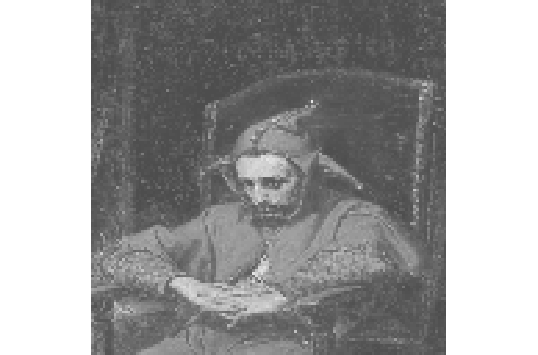
\includegraphics[width=0.7\textwidth]{128_128_stanczyk.png}\\[1ex]
  \Large Jan Matejko: \emph{Stańczyk} (1862)
\end{frame}

% --- Slide 2: Rank-10 (SVD) ---
\begin{frame}{SVD — Singular Value Decomposition, Mathematically optimal... but still a bit dreamy.}
  \centering
  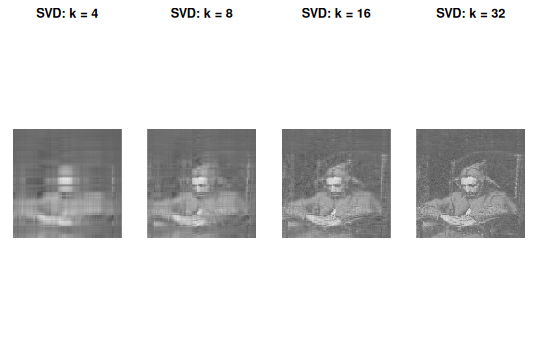
\includegraphics[width=1\textwidth]{decomposition_SVD_stanczyk.png}\\[1ex]
 \end{frame}

% --- Slide 3: CUR ---
\begin{frame}{CUR — Matrix Approximation, Fast and frugal... Stańczyk on a budget.}
  \centering
  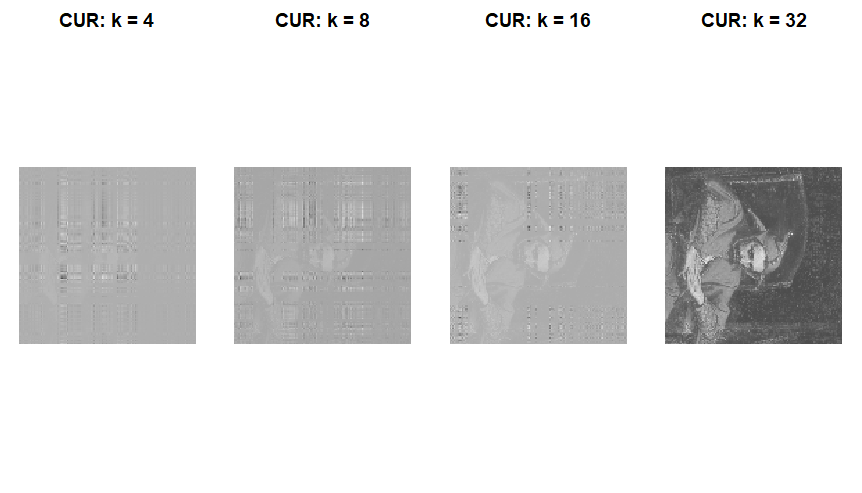
\includegraphics[width=1\textwidth]{decomposition_CUR_stanczyk.png}\\[1ex]
  \end{frame}

% --- Slide 4: NMF ---
\begin{frame}{NMF — Nonnegative Matrix Factorization, Pieces of the puzzle... Stańczyk in parts.}
  \centering
  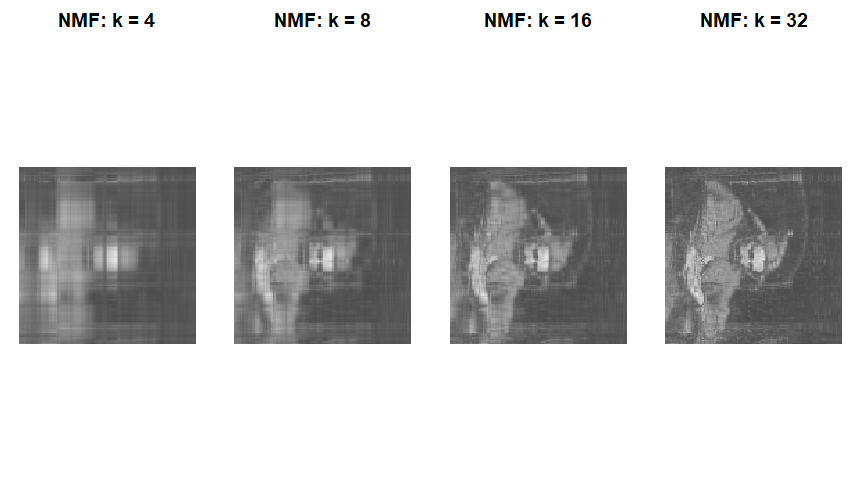
\includegraphics[width=1\textwidth]{decomposition_NMF_stanczyk.png}\\[1ex]
  \end{frame}

% --- Slide 5: Trailer slogans ---
\begin{frame}{Stay tuned...}
  \centering
  \Large Coming to your R console soon! \\
  \Large Starring: \textbf{SVD}, \textbf{NMF}, \textbf{CUR} \\
  \Large in the role of data approximations. \\
  \Large Grab your keyboard and join the show!
\end{frame}

\end{document}
